\chapter{App}
\section{Unity}
\label{sec:Unity}
Projekte in Unity setzen sich aus Szenen zusammen, in denen Objekte platziert sind. Diese Objekte besitzen Eigenschaften, die direkt im Unity-Editor gesetzt werden können, z.B. Position oder Material. Zusätzlich können die Objekte mit Skripten verbunden werden, die ihr Verhalten beeinflussen.

\subsection{Verzeichnisstruktur}
\label{sec:Verzeichnisstruktur}
Im Verzeichnis Assets innerhalb der Projekt-Root befinden sich im Wesentlichen alle externen Dateien, die für das Projekt benötigt werden. Es existieren folgende Unterverzeichnisse:

\begin{itemize}
  \item \_Scenes -- enthält die Szenen-Dateien der App, die im Unity-Editor bearbeitet werden können
  \item Audio -- enthält Sounddateien (Frage richtig beantwortet, Frage falsch beantwortet, Münze eingesammelt)
  \item Cardboard -- Verzeichnis des Cardboard SDK
  \item Font -- enthält den in der App verwendeten Font (Ubuntu)
  \item Graphics -- enthält das FH Wedel Logo zur Verwendung als App-Logo, sowie zur Verwendung als Normal-Map auf der Münze
  \item Materials -- enthält verwendete Texturen (für die Münze und die Ka\-me\-ra\-bild-Ebene)
  \item Plugins -- enthält verwendete Plugins; sowohl von Unity direkt (Android), als auch von uns (ZXing)
  \item Prefabs -- enthält zur mehrfachen  Verwendung erstellte Bausteine (der in der App verwendete Button)
  \item Resources -- enthält Ressourcen, die zur Laufzeit des Programms dynamisch geladen werden (die Münze und das Partikelsystem)
  \item Scripts -- enthält die verwendeten C\#-Dateien
\end{itemize}

\subsection{Szenen}
\label{sec:Szenen}
Die App besitzt vier Szenen:

\begin{enumerate}
  \item MainMenuScene
  \item HelpScene
  \item CameraScene
  \item QuestionScene
\end{enumerate}

Im Folgenden wird kurz erläutert welchen Zweck die Szenen dienen, welche Objekte sie enthalten und mit welchen Skripten sie zusammenhängen.

\subsubsection{MainMenuScene}
\label{subs:MainMenuScene}
Diese Szene dient als Einstiegspunkt der App und stellt das Hauptmenü dar. Wichtige Elemente der Szene sind das Canvas-Objekt, das drei Text-Objekte (für den Titel und die Anzeige des Spielfortschritts), sowie drei Buttons (Wechsel zur Kamera, Hilfe und Beenden) enhält. Das Canvas-Objekt ist mit dem Skript \texttt{MainMenuUi.cs} verknüpft, das die Liste aller Fragen aus der API lädt und die Interaktion mit den Buttons behandelt.

\subsubsection{HelpScene}
\label{subs:HelpScene}
Die HelpScene dient der Anzeige eines kurzen Erläuterungstextes innerhalb der App. Sie ähnelt dem Aufbau der MainMenuScene mit einem Canvas, in dem Text- und Button-Objekte liegen. Der Canvas ist mit dem Skript \texttt{HelpUi.cs} verknüpft.

\subsubsection{CameraScene}
\label{subs:CameraScene}
Die CameraScene ist dafür zuständig das aktuelle Kamerabild anzuzeigen und eventuell vorhandene QR-Codes im Bild zu erkennen und zu behandeln. Die Behandlung erfolgt entweder durch einen Szenenwechsel zur QuestionScene, oder durch das Anzeigen einer Münze oder eines Partikelsystems vor der Position des QR-Codes. Außerdem können in dieser Szene kurze Nachrichten an den Nutzer in Form einer Toast-Message angezeigt werden.

Die Szene enthält immer eine Ebene im 3D-Raum, auf die das Kamerabild projiziert wird, sowie einen Canvas mit einem Toast-Objekt. Weitere Objekte, wie die Münze oder das Partikelsystem, die sich vor den QR-Codes befinden, werden im Code erzeugt.

Da zu Beginn der Entwicklung der Fokus mehr auf der Verwendung des Google Cardboard lag, befindet sich die Ebene in der Objektstruktur direkt unterhalb der \emph{Main Camera} im \emph{Head} des \emph{CardboardMain}-Objekts. Somit bewegt sich die Ebene stets mit dem Kopf des Nutzers mit und das Kamerabild befindet sich immer direkt vor der Engine-Kamera.

Die gesamte Logik der CameraScene wird durch \texttt{CameraScript.cs} gehandhabt, welches mit der Kamerabild-Ebene verknüpft ist.

\subsubsection{QuestionScene}
\label{subs:QuestionScene}
Die QuestionScene stellt die zum gescannten QR-Code passende Frage, sowie deren Antwortmöglichkeiten dar. Die Reihenfolge der Antworten wird bei jedem Aufruf einer Frage zufällig durchgemischt. Der Nutzer kann durch Tippen eine Antwort auswählen und erhält ein visuelles und akustisches Feedback, ob seine Wahl korrekt war. Auch diese Szene basiert im Kern auf einem Canvas, das Text-Objekte und Buttons enthält und mit dem Skript \texttt{QuestionUi.cs} verknüpft ist.

\section{Code-Dokumentation}
\subsection{QR-Code-Erkennung}
Über die Unity-Klasse \texttt{WebCamTexture} wird auf das aktuelle Kamerabild zugegriffen. Dieser Zugriff ist, wie bei anderen Unity-APIs auch, nur vom Main-Thread aus erlaubt. Um das Durchsuchen des Bilds von der Darstellung der App loszukoppeln erfolgt die QR-Code-Erkennung auf einem separaten Thread. Die Pixeldaten der Kamera werden in der \texttt{Update}-Methode des \texttt{CameraScript} (also einmal pro Frame) in einem Feld gespeichert. Der Thread liest kontinuierlich die Daten aus diesem Feld aus und versucht QR-Codes im Bild zu erkennen. Hierbei kommt die Bibliothek \emph{ZXing} zum Einsatz. Schließlich wird eine Sammlung mit erkannten QR-Codes mit den Ergebnissen aktualisiert (siehe \texttt{QrCodeCollection} und \texttt{QrCodeData}).

\subsection{QR-Code-Verarbeitung}
Ist bisher noch kein QR-Code im Sichtfeld der Kamera, wird der QR-Code im Anschluss an die Erkennung dekodiert. Basierend auf den enthaltenen Daten soll ein entsprechendes 3D-Objekt erzeugt und dargestellt, oder die Szene gewechselt werden. Das Programm befindet sich zu diesem Zeitpunkt nicht in dem Unity-Main-Thread. Daher kann nicht direkt ein Objekt angelegt werden. An dieser Stelle wird ein entsprechend markiertes \texttt{QrCodeData}-Objekt in die \texttt{QrCodeCollection} eingefügt. Die eigentliche Erzeugung des 3D-Objekts erfolgt in der \texttt{Update}-Methode des \texttt{CameraScript}s und somit auf dem Unity-Main-Thread.

Ist bereits ein QR-Code im Sichtfeld, wird seine Position anhand der neu erkannten Positiondaten aktualisiert. Auf Basis der neu erkannten Position wird eine Zielposition für das \texttt{QrCodeData}-Objekt berechnet.

\begin{figure}[!h]
  \centering
    \begin{subfigure}{0.42\textwidth}
      \centering
        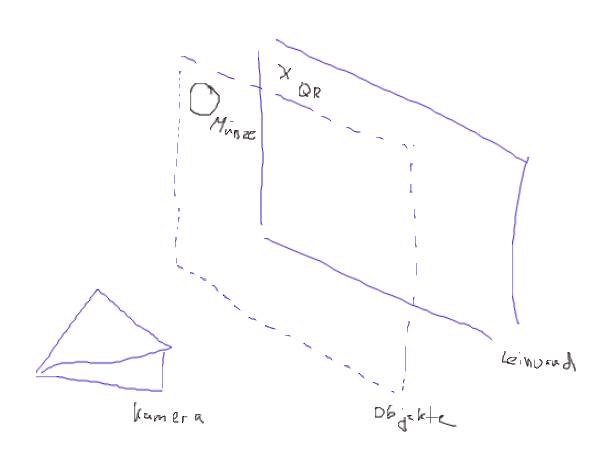
\includegraphics[width=\textwidth]{position_skizze_falsch}
      \caption{Naiver Ansatz}
    \end{subfigure}%
    \begin{subfigure}{0.42\textwidth}
      \centering
        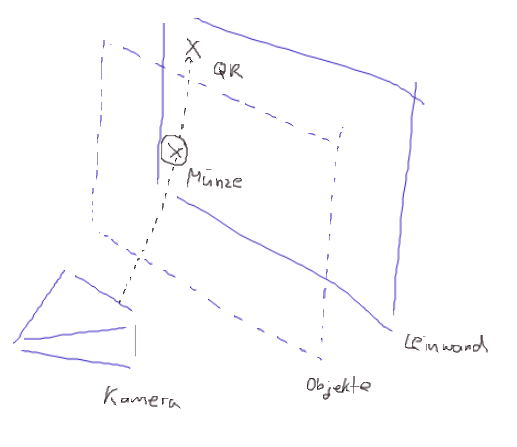
\includegraphics[width=\textwidth]{position_skizze_richtig}
      \caption{Korrekter Ansatz}
    \end{subfigure}
    \caption[Positionsberechnung der 3D-Objekte]{Positionsberechnung der 3D-Objekte. Links der naive Ansatz, rechts die korrekte Berechnung.}
    \label{fig:position_sketch}
\end{figure}

Bei der Berechnung der Positionierung muss beachtet werden, dass sich das Objekt nicht direkt auf der Leinwand, sondern auf einer gedachten Ebene davor befindet. Um zu gewährleisten, dass ein eingeblendetes Objekt korrekt vor dem QR-Code angezeigt wird, darf nicht die erkannte Position des QR-Codes übernommen werden. Stattdessen muss ein Strahl vom Augpunkt zur Position des QR-Codes auf der Leinwand geschossen werden. Der Schnittpunkt des Strahls mit der Objekt-Ebene ist die korrekte Position des 3D-Objekts.

Die Anpassung der Position zwischen aktueller und Zielposition wird in jedem Frame linear interpoliert, damit die Bewegung des 3D-Objekts flüssiger dargestellt wird. Leicht ungenaue Positionserkennung und eine handgeführte Kamera werden dadurch ausgeglichen.


\section{Google Play}
Wie eine App im Google Play Store veröffentlicht wird kann hier nachgelesen werden: http://developer.android.com/distribute/googleplay/start.html.

Zu beachten ist, dass man aus Unity ein \textbf{signiertes} APK für den Upload im Play Store exportiert. Dafür muss in Unity unter \emph{Edit \textrightarrow\ Project Settings \textrightarrow\ Player \textrightarrow\ Android Tab \textrightarrow\ Publishing Settings} ein existierender Keystore eingetragen oder ein neuer angelegt werden. Anschließend kann über \emph{File \textrightarrow\ Build Settings} ein Android Build gestartet werden, der den gewählten Keystore und Alias verwendet, um das Package zu signieren. Der Keystore muss unbedingt sicher aufbewahrt werden, da Updates für eine einmal veröffentlichte App nur mit dem selben Keystore und Alias erneut signiert werden können. Geht der Keystore verloren, muss auch die App im Play Store neu angelegt werden (mehr Details hier: http://developer.android.com/tools/publishing/app-signing.html\#secure-key).
